\chapter{Presentation-Abstraction-Control}

\section{Summary}
Das Presentation-Abstraction-Control (PAC) Pattern definiert eine Struktur für interaktive Software Systeme in Form einer Hierarchie von zusammenarbeitenden Agents. Jeder Agent ist dabei für einen spezifischen Teil der Funktionalität der Software zuständig. Ein Agent besteht aus den Komponenten Presentation, Abstraction und Control. Diese Unterteilung separiert den Mensch-Computer-Interaktions Aspekt des Agents von seinem funktionellen Kern und der Kommunikation mit anderen Agents.
\section{Context}
Entwicklung einer Interaktiven Applikation mit Einsatz von Agents.
\section{Problem}
Interaktive Systeme können oft als eine Sammlung von zusammenarbeitenden Agents gesehen werden. In solch einem System ist jeder Agent auf eine bestimmte Aufgabe spezialisiert, und alle Agents zusammen bilden das System. Folgende Forces haben einen Einfluss auf die Lösung:
\begin{itemize}
	\item Agents haben oft ihren eigenen State bzw. ihre eigenen Daten. Um zusammenarbeiten zu können brauchen die Agents einen Mechanismus zum Austausch von Daten, Messages und Events.
	\item Interaktive Agents bieten oft ihr eigenes Interface.
	\item Systeme entwickeln sich über die Zeit. Änderungen an einzelnen Agents oder das hinzufügen solcher sollte keinen Effekt auf das gesamte System haben.
\end{itemize}
\section{Solution}
Strukturierung der interaktiven Applikation als eine baumartige Hirarchie von PAC Agents, wobei es einen Top-Level Agent, mehrere Intermediate-Level Agents und noch mehr Bottom-Level Agents gibt. Jeder Agent ist abhängig von allen Agents auf einem höheren Level rauf bis zum Top-Level Agent. Im folgenden die Aufgaben der Level:
\paragraph{Top-Level Agent} Bietet den funktionellen Kern des Systems
\paragraph{Bottom-Level Agents} Repräsentieren in sich geschlossene semantische Konzepte auf denen User des Systems arbeiten können. 
\paragraph{Intermediate-Level Agents} Repräsentieren entweder Kombinationen oder Beziehungen zwischen Low-Level Agents. 
Ein Agent ist in die Komponenten Presentation, Abstraction und Control unterteilt. Die Presentation Komponente bietet das sichtbare Verhalten des PAC Agent. Von der Abstraction Komponente wird das Datenmodell verwaltet, sie bietet Funktionalität welche auf diesen Daten operiert. Die Control Komponente verbindet Presentation und Abstraction, und bietet zusätzlich Funktionalität die dem Agent ermöglicht mit anderen Agents zu kommunizieren.
\subsection{Structure}
Folgende Grafik zeigt die oben erwähnten drei Levels für eine Beispiel Applikation die als Informationssystem für Politische Wahlen dient. 
\begin{figure}[H]
	\centering
	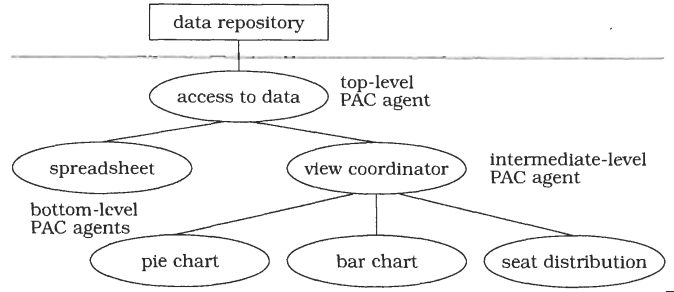
\includegraphics[width=0.6\textwidth]{figures/04-pac-1}
	\caption{PAC Level in einer Beispiel Applikation}
\end{figure}
Wie man sieht gibt es einen Top-Level PAC Agent. Dieser ist wie jeder Agent in die drei Komponenten unterteilt. Die Presentation Komponente hat auf diesem Level kaum Verantwortlichkeiten. Sie hat vieleicht UI Komponenten die von der gesamten Applikation verwendet werden, oder sie fällt ganz weg. 
Die Control Komponente auf diesem Level ermöglicht Lower-Level Agents auf die Services dieses Layers zuzugreifen, ausserdem koordiniert sie die Hierarchie der Agents und hält Informationen über die Interaktion des Users mit dem System.
Die Abstraction Komponente bietet in der Beispiel Applikation eine Schnittstelle zum darunter liegenden Daten Repository, es werden ausserdem Algorithmen zur Berechnung von Vorhersagen etc. hier implementiert. \\
Bottom-Level PAC Agents präsentieren auf der Presentation Komponente eine spezifische View der Daten, und bieten Zugriff auf alle Funktionen die ein User auf diesen tätigen kann. Die Abstraction Komponente ist ebenfalls für die Datenhaltung zuständig, allerdings sind hier keine anderen Agents davon abhängig. Die Control Komponente dient als Adapter zwischen Presentation und Abstraction, ausserdem kommuniziert Sie mit den höher gelegenen Agents. \\
Intermediate-Level PAC Agents können zwei verschiedene Rollen haben, composition oder coordination. In der composition Role führen sie die Bottom-Level Agents zu einer Abstraktion zusammen. In der coordination Role sind sie für die Konsistenz zwischen den Lower-Level Agents zuständig. 

\section{Consequences}
\begin{itemize}
    \pro{Separation of Concerns}
    \pro{Support for Change and Extention}
    \con{Erhöhte System Komplexität}
	\con{Komplexe Control Komponente}
	\con{Effizienz}
	\con{Anwendbarkeit}
\end{itemize}

\section{Known Uses}
\begin{itemize}
	\item Netzwerk Verkehr Management System
	\item Mobile Robot
\end{itemize}

\section{Relationships}
\begin{itemize}
	\item \textit{Model-View-Controller} 
\end{itemize}

\section{Exam Questions}
\begin{itemize}
  \item Behauptung: dies ist eine Behauptung? (Lösung)
    \item Frage: Dies ist eine Frage? (Lösung)
\end{itemize}
